\documentclass{article}
\usepackage{fullpage}
\usepackage{tikz}

\usepackage{questions}		% Option "exam" suppresses everything like names, feedback, correct answers, etc.
						% and puts each question on its own page
						% Option "key" displays questions, correct answers (if marked), and feedback (e.g.
						% full solutions).
						% for simple \usepackage{questions} with no options, everything is displayed, 
						% including notes and keywords (which presumably you'd not ever want to 
						% put on documents given to students)
						% option "byqref" lets you hide questions in your document until you later show them
						% with a call to \qref{name} (where name is the name of your question)
						% this gives the ability to pull individual questions from banks

\begin{document}

\begin{question}[2018.S.7]  %Question name (in this case 2018.S.17) is optional but important for question banking
The region in the plane bounded on the right by the curve $x = \cos y$, on the left by $x=0$, and on the bottom by $y = 0$ is revolved around the $x$-axis. Compute the volume of the resulting solid.
\begin{multiplechoice} 
\choice{$\displaystyle \pi^2$}
\choice{$\displaystyle \pi(\pi-1)$}
\choice[correct]{$\displaystyle \pi(\pi - 2)$} \choicebreak %normally the package tries to arrange answers automatically
								% but you can manually add \choicebreak if you want to force a 
								% new line for multiple choice answers
\choice{$\displaystyle \pi(\pi-3)$}		% marking the right answer as [correct] is important for question banking
\choice{$\displaystyle \pi(\pi-4)$}
\choice{none of these}
\end{multiplechoice}
\begin{keywords}volumes of revolution, shell method\end{keywords}
\end{question}


\scratchbreak  % If package is used with option "exam", \scratchbreak inserts a blank page (otherwise does nothing)


\begin{question}[2016.6]
\begin{image}				% At the start of a question you can include an image. It is automatically
						% left-justified and the rest of the question is properly wrapped.
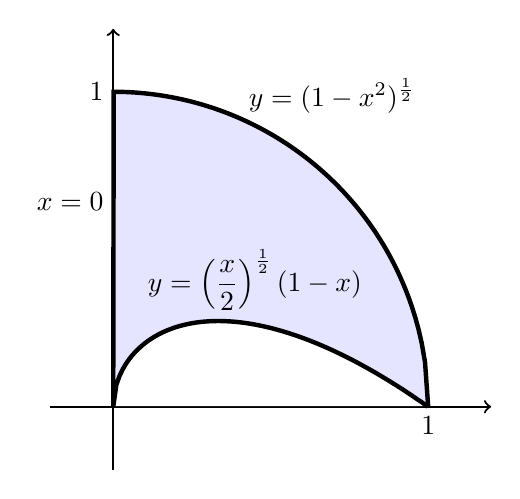
\begin{tikzpicture}[scale=4]
\draw [thick, ->] (0,-0.2) -- (0,1.2);
\draw [thick,->] (-0.2,0) -- (1.2,0);
\draw  [ultra thick, domain=0:1, samples=100, fill=blue!10!white] plot (\x,{sqrt( 0.5 * \x * (1- \x)*(1-\x))})  [domain=0:1, samples=100] plot ({1-\x},{sqrt( 1 - (1-\x)*(1-\x))}) -- (0,0) ;
\node [below] at (1,0) {$1$};
\node [left] at (0,1) {$1$};
\node [above] at (0.45,0.275) {$\displaystyle y = \left( \frac{x}{2} \right)^{\frac{1}{2}} (1-x)$};
\node [above right] at (0.4,0.9) {$\displaystyle y = (1-x^2)^{\frac{1}{2}}$};
\node [left] at (0,0.65) {$x = 0$};
\end{tikzpicture}
\end{image}
Find the volume of the solid of revolution obtained by rotating the planar region indicated below around the axis $y = 0$. 
\begin{multiplechoice}
\choice{$\displaystyle \frac{\pi}{8}$}
\choice{$\displaystyle \frac{2\pi}{8}$}
\choice{$\displaystyle \frac{3\pi}{8}$}
\choice{$\displaystyle \frac{4\pi}{8}$}
\choice[correct]{$\displaystyle \frac{5\pi}{8}$}
\choice{$\displaystyle \frac{6\pi}{8}$}
\end{multiplechoice}
\begin{comments}
\[ \begin{aligned} \int_0^1 \pi \left( (1-x^2) - \frac{x}{2}(1-x)^2 \right) dx & = \int_0^1 \pi \left(1  - \frac{x}{2}  - \frac{x^3}{2} \right) dx \\ & = \pi \left( 1 - \frac{1}{4} - \frac{1}{8} \right) = \frac{5 \pi}{8} \end{aligned} \]
\end{comments}
% There are four types of things you can place at the end of a question, after multiple choice options
% \begin{comments}...\end{comments} is for general comments that you'd like all students to see.
% \begin{feedback}...\end{feedback} is for comments you'd make to someone who got a wrong answer.
% \begin{praise}...\end{praise} is for comments you'd make to a student with the correct answer.
% \begin{notes}...\end{notes} are information for yourself or other instructors (e.g., is it tricky in some way)
% \begin{keywords}...\end{keywords} is what it sounds like
\end{question}


% If you add the option "byqref" to the question package and uncomment the lines below, you'll get basic
% question bank functionality. You can tell it's working because we've referred to them in reverse.
% You'll also get a blank first page if you also have the "exam" option, i.e., \usepackage[exam,byqref]{questions} ,
% and you left the \scratchbreak above

%\qref{2016.6}
%\qref{2018.S.7}



\end{document}